\phantomsection
\chapter{Motivations}

\noindent A facial expression is a visible manifestation of the effective state, cognitive activity, intent, personality, and psychopathology of a person \cite{DON99}; facial expressions play a significant role in human dialogue and interaction. Indeed, facial expressions carry more informations than mere speech, informations on which humans can relay for interaction. Facial expressions have a considerable effect on a listening interlocutor; a speaker facial expressions accounts for about 55 percent of the effect, 38 percent of the latter is conveyed by voice intonation and 7 percent by the spoken words \cite{PAN00}.
\newline

\noindent Since Antiquity, researchers have been interested in emotion and more particularly in emotion recognition. But one of the important studies on facial expression analysis impacting on the modern day science of automatic facial expression recognition was the work carried out by Charles Darwin \cite{BET12}. In 1872, Darwin wrote a treatise that established general expression principles and expression means for both humans and animals \cite{DAR04}. He also classified various kinds of expressions. This can be considered as the beginning of facial expression recognition.
\newline

\noindent Now, with the emergence of new technologies and computers, research is now focused on computer-based automatic facial expression recognition. Because facial expressions are major factors in human interaction, this research field will broaden the domain of Human-Machine Interaction. Indeed, emotion recognition will enable computers to be more responsive to users' emotions, and allow interactions to become more and more realistic. 
\newline

\noindent Another domain where facial expression recognition is an important issue is robotics. With the advances made in robotics, robots nowadays tend to mimic human emotion and react as as human-like as possible, especially for humanoid robots. However, since robots are being more and more present in our daily lives, they need to understand and recognize human emotions.
\newline

\noindent A lot of real time applications in the robotics field have already been created. For example, Bartlett et al. have successfully used their face expression recognition system to develop an animated character that mirrors the expressions of the user (called CU Animate) \cite{BAR03}. They have also been successful in deploying the recognition system on Sony's Aibo Robot and ATR's RoboVie \cite{BAR03}. Another interesting application has been demonstrated by Anderson and McOwen, called "EmotiChat" \cite{AND06}. It is a regular chatroom, except the fact that their facial expression recognition system is connected to the chat and convert the users' facial expressions into emoticons. Because facial expression recognition systems' robustness and reliability are constantly increasing, lots of innovative applications will appear.
\newline

\noindent There are also various other domains where emotion recognition can be used: Telecommunications, behavioural science, video games, animations, psychiatry, automobile safety, affect-sensitive music jukeboxes and televisions, educational software, etc \cite{BET12}.
\newline

\noindent Our project focuses on real-time facial expression recognition from a video stream. Indeed, facial expression recognition can be performed \textit{statically} on input images, or \textit{dynamically} on video sequences. Systems can also be \textit{obtrusive}, or \textit{non-obtrusive}, the former based on a device mounted on the user's head or body, therefore following each of his movements and perform facial expression recognition without much losses, while the latter can encounter difficulties if the user is not properly situated. However, non-obtrusive systems allow more natural user interactions. We chose our system to be non-obtrusive, and will detail further its setup in the next section.
\newline

\phantomsection
\section{Environment Setup}

\vspace{\baselineskip}
\noindent Our system will use the camera embedded into a Microsoft Kinect to record the user's video input, and we will consider a casual use of the camera, with the user sitting in front of the computer, the camera being next to it, as seen in \textbf{\color{red} Insert figure \& ref to figure}. This camera provides a 640$\times$480 pixels frame resolution, while recording at 30 FPS.
\newline

\noindent For development and training purposes we will use some pre-existing emotion datasets, in order to validate the efficiency of the system before testing it in real conditions.
\newline

\phantomsection
\section{Emotion Datasets}

\noindent Databases are very important for facial expression recognition system.
\newline

\noindent Using the same databases for studies that aims to improve existing systems is very useful. It allows to compare he results and to see if the new system is indeed better than the existing one. A lot of research studies work is based on the same databases than previous studies in order to compare the efficiency of their algorithm.
\newline

\noindent But databases are hard to construct. It has to fill all the requirements and that is why most of the work on facial expression recognition is based on existing databases. The hardest requirement to fill is to have a standardized database. Most of the actual databases use posed expressions and not spontaneous expression, and both are very different. New versions of the databases are coming out with spontaneous expressions in order to be more complete. Even with this transition from posed expressions to spontaneous expressions, there are other requirements that should be respected to have a database standardized for training and testing. It should contain images and video sequences and both should be of different resolutions. It should also contain people displaying expressions under different conditions: it could be change in the lighting, occlusions or rotations of the head \cite{BET12}.  
\newline

\noindent Following are the databases that will be used to test this facial expression recognition system. These are part of the databases that are popular, freely available and mostly used in the past few years.
\newline

\subsection{Japanese Female Facial Expression Database (JAFFE)}

\vspace{\baselineskip}
\noindent The database contains 213 images of 7 facial expressions (6 basic facial expressions: happy, angry, afraid, disgusted, sad, surprised + 1 neutral) posed by 10 Japanese female models. Each expression has been photographed three or four times. Each image has been rated on 6 emotion adjectives by 60 Japanese subjects. The database was planned and assembled by Miyuki Kamachi, Michael Lyons, and Jiro Gyoba \cite{JAFFE}.
\newline

\noindent This DB contains only posed expressions. The photos have been taken under strict controlled conditions of similar lighting and with the hair tied away from the face \cite{BET12}. 
\newline

\noindent Following are an example of images contained in the database. Here the subject is a woman and she displays 7 different emotional expressions (neutral, happy, angry, afraid, disgusted, sad, surprised): 
\newline

\vspace{\baselineskip}
\begin{center}
\noindent 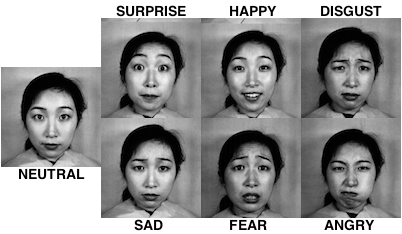
\includegraphics[scale=0.8]{figures/jaffe_7facialexpressions} 
\newline
\end{center} 

\subsection{Karolinska Directed Emotional Faces Database (KDEF)}

\vspace{\baselineskip}
\noindent The Karolinska Directed Emotional Faces (KDEF) is a set of totally 4900 pictures of human facial expressions of emotion. The material was developed in 1998 by Daniel Lundqvist, Anders Flykt and Professor Arne Ohman at Karolinska Institutet, Department of Clinical Neuroscience, Section of Psychology, Stockholm, Sweden \cite{KDEF}.
\newline

\noindent The material was originally developed to be used for psychological and medical research purposes. More specifically material was made to be particularly suitable for perception, attention, emotion, memory and backward masking experiments. Hence, particular attention was for instance paid to create a soft, even light, shooting expressions in multiple angles, use of uniform T-shirt colors, and use of a grid to center participants face during shooting, and positioning of eyes and mouths in fixed image coordinates during scanning \cite{KDEF}.
\newline

\noindent The set contains 70 individuals (35 males and 35 females), ranging from 20 to 30 years, each displaying 7 different emotional expressions (neutral, happy, angry, afraid, disgusted, sad, surprised),
each expression being photographed (twice) from 5 different angles (-90, -45, 0, +45, +90 degrees: i.e. full left profile, half left profile, straight, half right profile, full right profile)  \cite{KDEF}.
\newline

\noindent Following are an example of images contained in the database. Here the subject is a woman photographed from a straight angle and she displays 7 different emotional expressions (neutral, happy, angry, afraid, disgusted, sad, surprised): 
\newline

\vspace{\baselineskip}
\begin{center}
\noindent 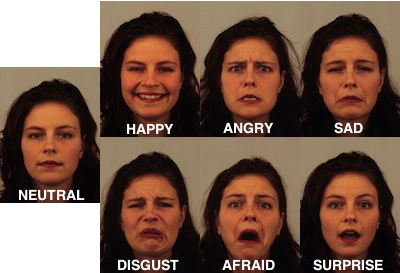
\includegraphics[scale=0.7]{figures/kdef_7facialexpressions} 
\newline
\end{center} 

\subsection{Montreal Set of Facial Displays of Emotion Database (MSFDE)}

\vspace{\baselineskip}
\noindent The database consists of emotional facial expressions by men and women of European, Asian, and African descent. Each expression was created using a directed facial action task and all expressions were FCAS coded to assure identical expressions across actors \cite{MSFDE}.
\newline

\noindent The set contains expressions of happiness, sadness, anger, fear, disgust, and embarrassment as well as a neutral expression for each actor. All expressions have been morphed into 5 different levels of intensity \cite{MSFDE}.
\newline

\noindent Following are an example of images contained in the database. Here the subject is an african woman and she displays 7 different emotional expressions (neutral, happy, angry, afraid, disgusted, sad, ashamed): 
\newline

\vspace{\baselineskip}
\begin{center}
\noindent 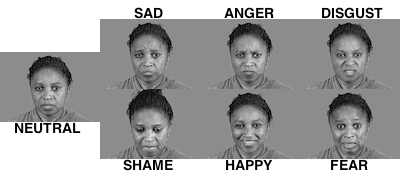
\includegraphics[scale=0.9]{figures/msfde_7facialexpressions} 
\newline
\end{center} 






